
\documentclass[11pt]{article}
\usepackage[margin = 1in]{geometry}
\usepackage[none]{hyphenat}
\usepackage{fancyhdr}
\usepackage{graphicx}
\graphicspath{{./images/}}
\usepackage{float}



\pagestyle{fancy}
\fancyhead{}
\fancyfoot{}
\fancyhead[L]{\slshape \MakeUppercase{Term Project}}
\fancyhead[R]{\slshape Mason Edmison}
\fancyfoot[C]{\thepage}

%%%%
% hack to remove indent
\newlength\tindent
\setlength{\tindent}{\parindent}
\setlength{\parindent}{0pt}
\renewcommand{\indent}{\hspace*{\tindent}}
%%%%

\begin{document}

\begin{titlepage}
\begin{center}
\Large{\textbf{Term Project}} \\
\Large{\textbf{CS 710 - Artificial Intelligence}} \\

\vfill
\line(1,0){400} \\

\Large{\textbf{Coreference Resolution in Biomedical Text:}} \\
\Large{\textbf{Improving Performance with Ontologies and Domain Specific NER}} \\

\line(1,0){400}\\
\vfill
Mason Edmison\\
University of Wisconsin-Milwaukee\\
12/10/2019
\end{center}
\end{titlepage}

\section{Introduction}
For my final project, I built a biomedical coreference resolution system using python open-source libraries. Coreference Resolution is a classical natural language processing problem. It is considered to be a hard and important problem as there are many applications that could benefit or have benefited from coreference resolution. Some of those applications are: question answering, text summarization, information extraction, and machine translation.

\section{Recent Work}

\subsection{Coreference Resolution}
Corefence resolution is a natural language processing problem where the task is to indentify which mentions in a text refer to the same real-world entity. 

\begin{figure}[h]
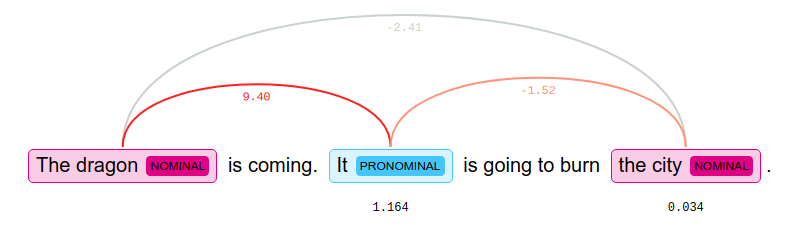
\includegraphics[width=8cm]{coref_vis}
\centering
\caption{Example of resolving coferring expression \textit{it} to antecedent \textit{dragon}}
\end{figure}

To better isolate specific sub-tasks within coreference resolution, we can consider the generic algorithm for anaphora and coreference resolution proposed by Ng et al., 2002. Algorithms and techniques described in this paper will use different implementations of these sub-tasks to improve the performance of resolving coreffering expressions. 
\begin{enumerate}
\item \textbf{Identification of referring expressions} Identify all noun phrases in the text. 
\item \textbf{Characterization of referring expressions} Composed of two sub-tasks: first, define a representation of a discourse entity. This representation determines the knowledge regarding a discourse entity that the algorithm needs in order to perform the remaining steps. Second, compute the information specified in the representation for each entity. 
\item \textbf{Anaphoricity determination} Determine whether a discourse entity is anaphoric or not. Non-anaphophoric entities, do not posses an antecedent and that algorithm will not search for these entitites. 
\item \textbf{Generation of antecedent candidates} Once a NP is determined to be anaphoric, the algorithm indentifies scope of the NP and gathers those NPs that falling with its scope to generate a list of canidate antecedents for it.
\item \textbf{Filtering} Remove unreasonable canidate antecedents for each anaphoric noun phrase. Can be based off of a set of rules or hard constraints. This step reduces the amount of processing that needs to be performed by the algorithm.
\item \textbf{Scoring/ Ranking} Score that indicates the likelihood that two NPs co-specify.
\item \textbf{Searching/ Clustering} Select an antecedent for a given anaphor from the list of canidate antecedents returned by the previous step. If this list is empty then no antecedent will be selected for this anaphor. 
\end{enumerate}


\subsection{Neural Network Systems}
Since this task requires knowledge at all levels of language processing, including lexical, syntactic, semantic, and world knowledge, success in this problem is indicative of advancement of language technologies. Appropriately, due to advancements in computational power, reinforcement learning, and semantic representation of words, coreference resolution has experienced a revival of sorts with many performant systems proposed in recent times. More specifically, Neural Network based coreference systems employing entity-level information and reinforcement learning have produced scores outperforming the previous state-of-the-art. An example of such a system is the Deep Reinforcement Learning system  proposed by Clark and Manning(2016). \\

\subsection{Deep Coref}
The deepcoref system is a deep neural network that builds distributed representations of coreference clusters using entity-level information and, using slack-rescaled ranking loss, learns when resolving coreference clusters is desirable. To gain better intuition of this system, it is better to think of this network comprising three sub-networks: mention-pair encoder, cluster-pair encoder, cluster-ranking model. \\
The mention pair encoder produces distributed representations for pairs of mentions by passing relevant features through a feed forward neural network. The cluster pair encoder produces distributed representations of pairs of clusters applying a combination of a max and average pooling operation. The cluster ranking model then scores pairs of representations through a single neural network. \\
Also, a mention-ranking model is trained that scores a pair of mentions through a single layer NN in which its output is used to prune clusters not to be considered by the cluster ranking model. Its output also functions as parameters used to initialize the cluster ranking model. \\

\begin{figure}[h]
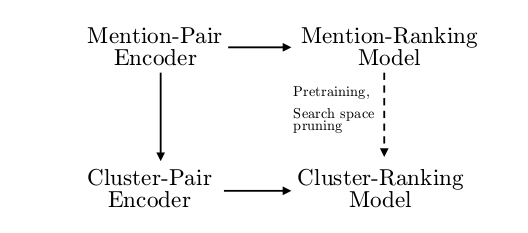
\includegraphics[width=8cm]{deepneural}
\centering
\caption{System Architecture defined of \textit{deep coref}.}
\end{figure}

\subsection{Open-Source Implementation}
Though the python source code from \textit{deepcoref} is publically available (Clark and Manning, 2016), it is reliant on StanfordCoreNLP components implemented in Java and is not optimized for speed\footnote{The \textit{deepcoref} system takes roughly 7 days to train on the CoNLL dataset on a GTX Titan GPU.}. So instead, I used the neuralcoref library for this project - an open-source cython library built by \textit{Hugging Face}\footnote{github repository found at https://github.com/huggingface/neuralcoref.}. Neuralcoref is greatly inspired by Clark and Mannings coreference system being that it builds mention vectors using the features proposed in the original paper as well as utilizes the slack rescaled ranking loss when ranking clusters\footnote{Regarding the algorithm proposed in section 2.1, these correlate to steps 2 and 6, respectively}. It is a SpaCy pipeline extension which provides great flexibility as we can introduce different language models and other pipeline components (EntityLinker, Named Entity Recognition, etc.). Neuralcoref ships pretrained on the ConLL 2012 dataset and with tuned word vectors trained on the OntoNotes 5.0 dataset. \\

\section{Dataset and Baseline Evaluation}
To evaluate the performance of this system, I used the annotated coreference resolution dataset from the 2011 BioNLP shared task. The goal of this shared task is to find anaphoric expressions to proteins. The annotated data includes 2,300 pubmed abstracts with corresponding protein and gene annotations as well as coreference cluster annotations. Given that the neuralcoref library evaluates performance based off a file in the tabular CoNLL format, I wrote an evaluation script that closely follows the ‘match’ guidelines outlined in the shared task\footnote{Writing these custom evaluation scripts proved to be quite helpul when investigating why and where the system was performing poorly.} \\
The system was evaluated using F1, precision, and recall scores. These metrics are calculated by comparing predicted cluster pairs vs gold annotated cluster pairs. A true postive is counted when a  predicted cluster comprises mentions of which both mentions are either within a minimum span of a gold mention\footnote{Some mentions in the annotated text have a minimum span that \textit{must} be included in the mention span. These minmum spans are generally genes or proteins that exist within a larger span.} or that a mention subsumes a gold mention of a gold cluster. 
To establish a baseline evaluation, I used the SpaCy \textit{en\_core\_web\_md} model with neuralcoref's default parameters (see table \ref{tab:baseline}). \\  
\begin{table}[h]
    \centering
 \begin{tabular}{||c c c c||} 
 \hline
  &  Prec.  & Rec. & $F1$ \\ [0.5ex] 
 \hline\hline
     SpaCy Web Md & 15.15\% & 8.37\% & 10.72\% \\ 
 \hline
\end{tabular}
\caption{Baseline evaluation score}
\label{tab:baseline}
\end{table}

\section{Possible Improvements}
Given a baseline performance score, I chose to focus on introducing domain-specific named entity recognition (Choi et al., 2014), dependency parsing, word vectors as well as ontologies to improve performance. Libraries I used to introduce these were: 
\begin{itemize}
    \item Word Vectors: BioWordVec - 200 dimension word vectors trained using a Fasttext vectorization algorithm on large corpus consisting of pubmed abstracts
    \item NER and dependency parsing: SciSpaCy which provides full SpaCy pipelines trained on biomedical text. 
    \item Ontologies: Sanaphor - open-source StanfordNLP implementation that uses ontologies to merge and split clusters in the last step of the (step 7) of the generic coref algorithm.
    \end{itemize}

\section{Modifications and Implementation}
The vanilla SciSpacy models provide 'generic' named entity recognition meaning that all entities found within text are annotated with the label ENTITY. SciSpacy also provides NER modules trained on different corpora (craft, jnlpba, bc5cde, bionlp13). For the particular task of identifying proteins and genes, I built a complete SciSpacy model using a NER module trained on the JNLPBA corpus which provides entity types DNA, CELL\_TYPE, CELL\_LINE, RNA, PROTEIN. To allow neuralcoref to 'accept' these entities within the rule-based mention detection, I had to add these entity types to the ACCEPTED\_ENTS constant\footnote{The forked neuralcoref repo with these modifications can be found at https://github.com/masonedmison/neuralcoref}. \\

Regarding word embeddings, neuralcoref uses static and tuned 50 dimensional word vectors that are used when calculating both mention embeddings as well as pair embeddings. Given that BioWordVec uses 200 dimensional vectors, I trained a new set of 50 dimensional word vectors on a corpus comprising 1 million Pubmed abstracts and a sampling of random walk sequences from a MeSh graph (Node2Vec). \\

\section{Results}
Using different language models and named entity recognition modules (table \ref{tab:improvements}), many spurious clusters were generated. My approach was to find the combination of a model and NER module that produced the best precision score and to implement different pruning techniques to further imrove this score. Pruning techniques employed were influenced by Prokofyev et al., 2015. Given the set of entities in a given document where entity $e \in \varepsilon$, a cluster was pruned if neither mention had an entity $\lnot \exists e \in \varepsilon$ or if a cluster comprised two mentions where entities $e_i, e_j \vert e_i \neq e_j$: 
The most performant combination was the use of the SciSpacy model, and pruning using a named entity recognition module trained on the JNLPBA corpus (see figure \ref{fig:false_pos}). 

\begin{figure}[h]
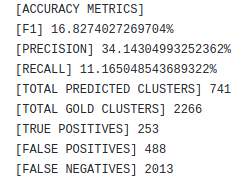
\includegraphics[width=4cm]{highest_prec}
\centering
\caption{Note the high number of False Positives even with pruning by entity type}
\label{fig:false_pos}
\end{figure}
\begin{table}[h]
    \centering
 \begin{tabular}{||c c c c||} 
 \hline
  &  Prec.  & Rec. & $F1$ \\ [0.5ex] 
 \hline\hline
     JNLPBA NER & 34.14\% & 11.17\% & 16.83\% \\ 
     SciSpacy MD & 29.86\% & 14.29\% & 19.33\% \\ 
     SciSpacy MD BWV & 2.02\% & 7.27\% & 3.16\% \\ 
 \hline
\end{tabular}
\caption{improved metrics using domain specific NER and language models}
\label{tab:improvements}
\end{table}

We see that in the third row of the table, very poor performance using word vectors trained on biomedical text. This can likely be attributed to the fact that the system was trained using the 50 dimensional google news vectors, so to see any performance gains using domain specific vectors, we would need to retrain the system using these vectors. \\

\section{Use Case}
To demonstrate a basic use case for this system, I wrote a simple command line script\footnote{coref\_annotater.py} that takes as input text or a .txt file and outputs text with coreferring expressions annotated with their antecedent. For a demonstration, please see the attached .mp4 video. This script could potentially be used as a preprocessing step for event extraction, information extraction, or text classifaction. Though currently in existence as a CLI, I envision it as a Rest API that could be easily accessed via POST request. In its current iteration, it currently takes other arguments: prune same literal form and prune by entity. Though it is quite simple, I think it demonstrates great potential. \\

\section{Conclusion and Next Steps}
Though I was able to improve the $F1$ and precision scores by 6\% and nearly 20\%, respectively, there are techniques that could be introduced that would likely further improve performance. Note that neuralcoref is trained on the CoNLL  dataset which is not domain-specfic. Given a large annotated biomedical dataset, training neuralcoref on this dataset would likely improve performance drastically. It would also be interesting to train neuralcoref with different word vectors, i.e. using word vectors trained on biomedical text such as BioWordVec or sequence embeddings such as BioBert or BioSentVec. \\
To evaluate the performance of the coreference system, I used generic implementations of the $F1$, precision, and recall scores, but a more thorough analysis considering mention detection as well as coreference specific metrics like $CEAF$ and $MUC$ would give a better indication of performance. \\ 

\newpage
\bibliographystyle{plain}
\bibliography{References}
\nocite{pilehvar-collier-2016-improved, choi-etal-2014-analysis, Prokofyev:2015:SOC:2942298.2942337, clark-manning-2016-improving}

\end{document} % end document
